
\myChapter{Riflessioni e conclusioni sui GA}
Quest'ultimo capitolo, volto a concludere la tesi, elenca rapidamente alcuni ambiti di applicazione dei GA, per poi terminare con una breve visione su quanto essi potranno essere utili in un futuro prossimo.
\section{I GA nei vari ambiti scientifici}
Gi\`a Goldman nella sua opera maggiormente nota \cite{goldberg1} inser\`i una esaustiva lista di campi di applicazione dei GA, i diversi ambiti andavano dalla biologia all'informatica, dall'ingegneria meccanica \cite{end1} all'image processing\cite{end2} ed al riconoscimento di pattern \cite{end3}, fino ad arrivare alla finanza\cite{end6} ed alla fisica. Abbiamo sempre ribadito quanto i GA siano flessibili, il loro ampio raggio d'impiego ne \`e la testimonianza pi\`u diretta.
%\vspace{3mm}
\begin{figure}[H]%
    \centering
    %\hfill
    \subfloat[Articoli per anno]{{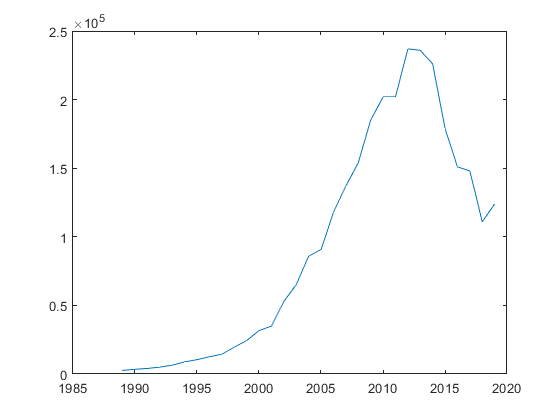
\includegraphics[width=0.5\linewidth]{Images/graph1.png}}}%
    %\qquad
    %\hfill
    \subfloat[Articoli per anno (cumulativi)]{{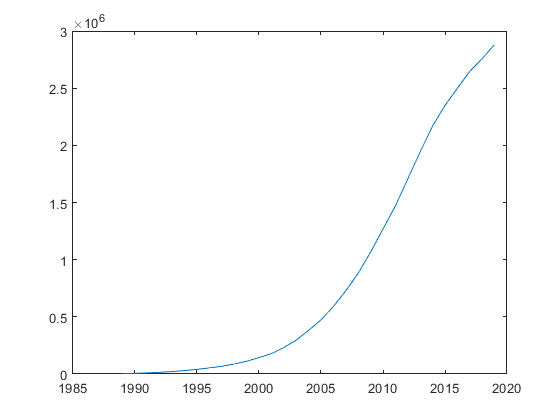
\includegraphics[width=0.5\linewidth]{Images/graph2.png}}}%
    %\hfill
    %\caption{Il problema del commesso viaggiatore, immagine trovata dal web}
    %\caption{Rappresentazione degli archi del grafo basato sul sudoku}
    \caption{Articoli per anno contenenti "Genetic Algorithm", fonte dei dati: Google Scholar}
    \label{fig:articles}%
\end{figure}
Dato il sempre crescente interesse verso il machine learning, i GA stanno ritornando sotto i riflettori anche se Goldberg per primo scrisse chiaramente sul loro uso in tale campo \cite{goldberg1} \cite{end7}; essendo il machine learning \cite{end4} \cite{end5}, e l'IA in generale, l'ambito pi\`u altisonante attualmente unito al sempre maggiore interesse da parte dell'aziende nell'assumere esperti in tali settori, fa comprendere quanto l'approccio mostrato in questa tesi possa risultare un importante tassello per chi prender\`a questa strada.
\section{Conclusioni e visioni sul futuro}
Per quanto ci possa addolarare affermare quanto segue dopo interi capitoli, dobbiamo senza dubbio ammettere che i GA non sono, allo stato attuale e dopo aver visto qualche implementazione, la soluzione migliore per i problemi di ricerca ed ottimizzazione; d'altro canto, abbiamo visto come la loro flessibilit\`a possa dare un grande vantaggio in certe situazioni (come sottolineato verso la fine del capitolo 5, risultano pi\`u efficaci in casi in cui il tempo sia il maggior discriminante).
\vspace{3mm}

Come il loro nome pu\`o suggerire, i GA sono sempre in continua evoluzione e, con la nostra piena speranza, usciranno pubblicazioni negli anni a venire che daranno nuove linfa vitale a questo metodo, la cui idea fondamentale rimane in ogni modo affascinante ed interessante.
%I GA non sono sicuramente, allo stato attuale, il miglior agloritmo in circolazione per quanto riguarda la ricerca e l'ott
%\section{}
\newpage